\chapter{INTRODUCTION}

\section{INTRODUCTION}
Real-time interactive voice communication over packet-switched networks has become the foundational backbone of modern global telecommunications. Over the past three decades, legacy circuit-switched infrastructure (such as the Public Switched Telephone Network, or PSTN) has been largely replaced by Voice-over-IP (VoIP) architectures, WebRTC media pipelines, and decentralized peer-to-peer audio protocols. Unlike non-interactive media streaming or traditional web browsing, real-time voice conversations impose exceptionally stringent physical and perceptual constraints on the underlying transport layer. Human conversation requires interactive latency to remain strictly below 150 milliseconds mouth-to-ear delay, as specified in ITU-T Recommendation G.114. If delay exceeds 200 to 250 milliseconds, conversational flow collapses into disruptive talker overlap and collision.

To achieve this low-latency delivery, voice engines uniformly rely on the User Datagram Protocol (UDP) at the transport layer, commonly paired with the Real-time Transport Protocol (RTP) and secured through the Secure Real-time Transport Protocol (SRTP). UDP avoids the connection establishment delays, retransmission buffering, and head-of-line blocking inherent to the Transmission Control Protocol (TCP). When an audio packet is delayed or dropped due to transient network congestion, retransmitting that packet over TCP is counterproductive: the retransmitted frame arrives dozens or hundreds of milliseconds after its scheduled playback deadline, rendering it useless for audio synthesis while simultaneously stalling the playback buffer for subsequent packets. 

Consequently, real-time voice architectures willingly accept an unreliable, lossy transport substrate. Audio codecs, most notably the standardized Opus codec (RFC 6716), are engineered to conceal lost frames via waveform extrapolation and low-bitrate forward error correction. However, this architectural dependence on UDP introduces a fundamental structural vulnerability when modern voice protocols must be upgraded to withstand the existential threat posed by quantum computation.

\section{THE QUANTUM THREAT AND POST-QUANTUM MIGRATION}
Every established secure voice transport today—including DTLS-SRTP in WebRTC, ZRTP, Signal's voice transport protocol, and TLS-based session control—relies on asymmetric public-key cryptography for endpoint authentication and session key exchange. These protocols depend almost exclusively on two mathematical problems: the integer factorization problem (exemplified by RSA) and the discrete logarithm problem over finite fields or elliptic curves (such as Diffie-Hellman, ECDH with Curve25519, and ECDSA).

In 1994, Peter Shor formulated a quantum algorithm that finds the prime factors of an integer and solves discrete logarithms in polynomial time $\mathcal{O}((\log N)^2 \log \log N \log \log \log N)$ \cite{shor1994algorithms}. On a sufficiently large fault-tolerant quantum computer running error-corrected physical qubits, classical asymmetric cryptography will cease to provide confidentiality or authenticity. While symmetric primitives such as AES-256 and ChaCha20 remain practically secure against quantum cryptanalysis—requiring Grover's algorithm to achieve a quadratic speedup that merely reduces 256-bit security to an effective 128-bit margin—asymmetric key negotiation mechanisms will be completely broken.

This cryptanalytic threat is not a distant prospective issue. Under the ``Harvest Now, Decrypt Later'' (HNDL) operational doctrine, nation-state intelligence agencies and well-resourced adversarial entities are actively intercepting and archiving petabytes of encrypted telecommunication traffic traversing international undersea cables and fiber-optic backbones. Even though adversaries cannot decipher the encrypted voice payloads today, any archived session key exchange negotiated via classical ECDH can be retroactively solved once cryptanalytically relevant quantum computers (CRQCs) become operational. For state secrets, diplomatic communications, proprietary corporate intelligence, and private civic discourse, confidentiality requirements routinely span twenty to thirty years. Encrypted voice sessions recorded today must therefore be secured with quantum-resistant key establishment mechanisms immediately.

In response to this imperative, the National Institute of Standards and Technology (NIST) conducted an intensive eight-year post-quantum cryptography standardization initiative, concluding in 2024 with the formal release of Federal Information Processing Standards (FIPS):
\begin{enumerate}
    \item \textbf{FIPS 203 (ML-KEM):} A module-lattice-based key encapsulation mechanism derived from CRYSTALS-Kyber, serving as the primary standard for quantum-resistant asymmetric key establishment \cite{nist_fips203}.
    \item \textbf{FIPS 204 (ML-DSA):} A module-lattice-based digital signature algorithm derived from CRYSTALS-Dilithium, designed for quantum-resistant digital authentication and integrity verification \cite{nist_fips204}.
\end{enumerate}

While these mathematical constructions withstand both classical and quantum cryptanalysis, their security relies on the hardness of lattice problems (specifically Module Learning With Errors, or M-LWE) over high-dimensional polynomial rings. This algebraic structure imposes a severe physical cost: cryptographic artifacts are orders of magnitude larger than their classical counterparts.

\section{THE CONFLICT: PQC OVERHEAD AND IP FRAGMENTATION}
The crux of this research arises from an irreconcilable conflict between post-quantum payload sizes and the fundamental constraints of datagram networks.

In classical communications, an elliptic-curve Diffie-Hellman key exchange (e.g., X25519) requires exchanging public keys of just 32 bytes, while an Ed25519 signature occupies 64 bytes. The entire classical mutual authentication handshake readily fits into a single, compact UDP packet well under 500 bytes.

In contrast, post-quantum primitives require substantial data transfer. In this work, we deploy the standard NIST security Category 3 parameter sets: ML-KEM-768 for key establishment and ML-DSA-65 for mutual identity authentication. The public parameters and cryptographic outputs exhibit the following dimensions:
\begin{itemize}
    \item \textbf{ML-KEM-768 Public Key:} 1,184 bytes
    \item \textbf{ML-KEM-768 Ciphertext:} 1,088 bytes
    \item \textbf{ML-DSA-65 Public Key:} 1,952 bytes
    \item \textbf{ML-DSA-65 Signature:} 3,309 bytes
\end{itemize}

A fully mutually authenticated handshake requires the calling entity (initiator) to transmit its ephemeral KEM public key, its long-term identity signature public key, and a signature proving ownership. The answering entity (responder) must reply with the encapsulated KEM ciphertext accompanied by a signature over the transcript. Summing these records yields an unprecedented handshake payload:
\begin{align}
    \text{Initiator HELLO} &= 1\ (\text{version}) + 1184 + 1952 + 3309 = 6,445\ \text{bytes} \\
    \text{Responder ACCEPT} &= 1\ (\text{version}) + 1088 + 3309 = 4,397\ \text{bytes} \\
    \text{Total Handshake Payload} &= 6,445 + 4,397 = \mathbf{10,842\ \text{bytes}}
\end{align}

This 10,842-byte security payload must traverse an Internet designed around a standard Ethernet Maximum Transmission Unit (MTU) of 1,500 bytes (and a minimum guaranteed IPv6 MTU of 1,280 bytes). When an application transmits a 6,445-byte or 4,397-byte datagram over standard UDP, the operating system kernel is forced to fragment the datagram at the IP layer.

\begin{figure}[htbp]
    \centering
    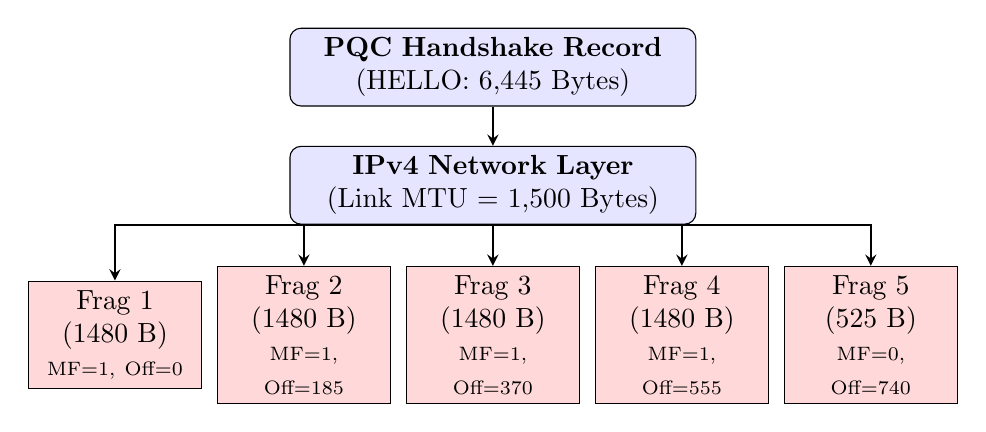
\begin{tikzpicture}[
        every node/.style={align=center},
        mainblock/.style={rectangle, draw, fill=blue!10, text width=14em, align=center, rounded corners, minimum height=2.4em},
        fragblock/.style={rectangle, draw, fill=red!15, text width=5.6em, align=center, minimum height=2.2em},
        conn/.style={thick, ->, >=stealth}
    ]
        \node [mainblock] (app) at (0, 3.0) {\textbf{PQC Handshake Record}\\(HELLO: 6,445 Bytes)};
        \node [mainblock] (ip) at (0, 1.5) {\textbf{IPv4 Network Layer}\\(Link MTU = 1,500 Bytes)};
        
        \node [fragblock] (f1) at (-4.8, -0.4) {Frag 1 (1480 B)\\{\scriptsize MF=1, Off=0}};
        \node [fragblock] (f2) at (-2.4, -0.4) {Frag 2 (1480 B)\\{\scriptsize MF=1, Off=185}};
        \node [fragblock] (f3) at (0, -0.4) {Frag 3 (1480 B)\\{\scriptsize MF=1, Off=370}};
        \node [fragblock] (f4) at (2.4, -0.4) {Frag 4 (1480 B)\\{\scriptsize MF=1, Off=555}};
        \node [fragblock] (f5) at (4.8, -0.4) {Frag 5 (525 B)\\{\scriptsize MF=0, Off=740}};

        \draw [conn] (app) -- (ip);
        \draw [conn] (ip.south) -| (f1.north);
        \draw [conn] (ip.south) -| (f2.north);
        \draw [conn] (ip.south) -- (f3.north);
        \draw [conn] (ip.south) -| (f4.north);
        \draw [conn] (ip.south) -| (f5.north);
    \end{tikzpicture}
    \caption{IPv4 Fragmentation of an Oversized PQC Handshake Datagram across an MTU of 1500 Bytes.}
    \label{fig:ip_frag_overview}
\end{figure}

As illustrated in Figure \ref{fig:ip_frag_overview}, transmitting the initiator's \texttt{HELLO} message results in five IP fragments, while the responder's \texttt{ACCEPT} produces three fragments, yielding eight physical packets for a single exchange. In IP fragmentation, reassembly occurs strictly at the receiving operating system's IP reassembly buffer. Crucially:
\begin{enumerate}
    \item \textbf{All-or-Nothing Reassembly:} UDP provides no selective acknowledgment or fragment-level retransmission. If even a single fragment among the eight is lost in transit, the destination kernel discards the remaining seven fragments upon reassembly timeout. The entire 10,842-byte handshake fails.
    \item \textbf{Exponential Failure Scaling:} Assuming independent packet loss probability $p$, the mathematical probability that an 8-fragment handshake successfully arrives intact is governed by:
    \begin{equation}
        P_{\text{survival}} = (1 - p)^8
    \end{equation}
    At a modest wireless packet loss of $p = 0.20$ (20\%), the survival rate collapses to:
    \begin{equation}
        P_{\text{survival}} = (1 - 0.20)^8 = (0.8)^8 \approx 0.1677\ \ (16.8\%)
    \end{equation}
    Over 83\% of call connection attempts fail completely.
    \item \textbf{Middlebox Pathologies:} Commercial network middleboxes—including NAT gateways, stateless stateful packet inspection firewalls, and Equal-Cost Multi-Path (ECMP) routers—routinely drop out-of-order IP fragments or non-zero offset packets to prevent reassembly buffer exhaustion attacks (e.g., Teardown and Rose attacks) \cite{shannon1984ipfrag}.
\end{enumerate}

Thus, naively injecting post-quantum cryptographic primitives into conventional UDP voice architectures catastrophically undermines the availability and survivability of the telecommunication service.

\section{PROJECT STATEMENT}
This thesis addresses the fundamental problem of network-layer fragmentation in post-quantum encrypted voice telecommunications. Specifically, this work formulates, implements, and evaluates a hybrid transport architecture that decouples control-plane security establishment from data-plane media streaming. By migrating the 10,842-byte post-quantum cryptographic handshake onto a reliable, stream-oriented TCP control channel while constraining encrypted Opus voice datagrams onto an unfragmented UDP data channel capped strictly at 1,200 bytes with the IP Don't-Fragment bit asserted, the system guarantees zero IP fragmentation while preserving real-time conversational latency.

\section{RESEARCH OBJECTIVES}
The primary technical and academic objectives of this project are:
\begin{enumerate}
    \item \textbf{Protocol Architecture Design:} Formulate a decoupled transport protocol (\textbf{HPQV}) combining reliable TCP control framing with low-latency, unfragmented UDP datagram streaming.
    \item \textbf{Post-Quantum Mutual Authentication:} Construct a secure cryptographic handshake deploying ML-KEM-768 and ML-DSA-65 with complete transcript binding (ADR-0002) and out-of-band identity pinning to prevent man-in-the-middle attacks.
    \item \textbf{Key Derivation and Directional Nonce Isolation:} Implement an HKDF-SHA256 expansion scheme that derives independent 32-byte session keys and distinct 4-byte directional nonce prefixes, eliminating symmetric cipher nonce reuse vulnerabilities in ChaCha20-Poly1305.
    \item \textbf{Enforced Datagram Invariant:} Establish an enforced application-level boundary of 1,200 bytes per voice packet, accompanied by explicit operating system configuration of the IP Don't-Fragment (DF) bit.
    \item \textbf{Audio Resilience Engine:} Integrate the Opus codec with in-band Low Bitrate Redundancy (LBRR) Forward Error Correction and a heap-based jitter buffer to mitigate packet drop and network jitter.
    \item \textbf{Full Userspace Prototype Implementation:} Develop a clean, modular implementation in Python 3.11 with low-level C bindings, complete with an interactive graphical user interface featuring real-time, in-call loss injection.
    \item \textbf{Multi-Tiered Empirical Benchmarking:} Validate the protocol across a reproducible, containerized testbed utilizing Linux Traffic Control (\texttt{tc netem}) for physical kernel measurement (Track 2) and NS-3 discrete-event network modeling (Track 3) against pure TCP and simulated QUIC baselines.
\end{enumerate}

\section{SCOPE AND BOUNDARIES}
To establish realistic boundaries for an academic B.Tech engineering thesis, the scope of this project is defined as follows:
\begin{itemize}
    \item \textbf{Target Topology:} Point-to-point (two-party) interactive voice communication over IPv4 local and wide-area networks. Multi-party conferencing (e.g., Selective Forwarding Units) is left for future expansion.
    \item \textbf{Identity Infrastructure:} Peer identity public keys are pinned out-of-band via trusted configuration files, matching the operational security models of WireGuard and SSH. Integration with an automated Public Key Infrastructure (PKI) or X.509 Certificate Authorities is excluded.
    \item \textbf{Cryptographic Primitives:} Evaluation focuses strictly on standardized lattice-based algorithms (ML-KEM-768 and ML-DSA-65). State-machine signature schemes (e.g., LMS/XMSS) and code-based schemes (e.g., Classic McEliece) are outside the primary prototype scope.
    \item \textbf{Network Environment:} Primary physical evaluations are conducted across virtualized network namespaces and containerized loopback interfaces with MTU pinned to 1,500 bytes to ensure rigorous, reproducible loss and delay control.
\end{itemize}

\section{ORGANIZATION OF THE REPORT}
The remainder of this report is structured as follows:
\begin{itemize}
    \item \textbf{Chapter 2 (Literature Survey):} Reviews theoretical foundations of post-quantum cryptography, real-time transport protocols (RTP, SRTP, WebRTC, QUIC), empirical studies on IP fragmentation middlebox pathologies, and audio quality assessment models.
    \item \textbf{Chapter 3 (System Architecture):} Presents the complete mathematical and architectural specification of the HPQV protocol, including wire framing, mutual authentication handshake mechanics, key ratcheting, and jitter buffer operation.
    \item \textbf{Chapter 4 (Implementation Details):} Details the software engineering architecture, core Python modules, C library bindings, socket-level flags, GUI development, and the 53-case automated verification test suite.
    \item \textbf{Chapter 5 (Experimental Methodology):} Describes the multi-tiered evaluation framework, containerized Docker environment, Linux NetEm configuration, NS-3 simulation calibration, and mathematical formulations for metrics.
    \item \textbf{Chapter 6 (Results and Discussion):} Analyzes empirical findings across fragment counts, handshake survival rates, connection setup latencies, FEC recovery SNR, and NS-3 comparative curves, followed by a critical engineering discussion.
    \item \textbf{Chapter 7 (Conclusion and Future Work):} Summarizes major research findings, validates project deliverables against initial objectives, and outlines future research avenues.
    \item \textbf{Appendices \& References:} Provides exhaustive wire format layouts, mathematical derivations, reproducible environment commands, core code listings, test suite catalogs, and APA references.
\end{itemize}
